\chapter{Architecture}
\index{architecture}
\minitoc

We will first look at various basic architectures and then try to decide on a final design.

\section{Logical reasoner (blackboard architecture)}
\label{sec:blackboard-architecture}
\index{architecture!blackboard}

This is an older design I explored around 2006, chiefly to put together several logic-based algorithms on a blackboard.  The following page is a schematic diagram showing various modules of the \textbf{logical sub-system}.

My intuition is that such a logical sub-system is essential to any AGI, but it should be built on top of a more basic, \textit{procedural} layer (cf \S\ref{sec:proc-subsumes-decl}, ``Procedural subsumes Declarative'').

\begin{figure}[H]
\centering
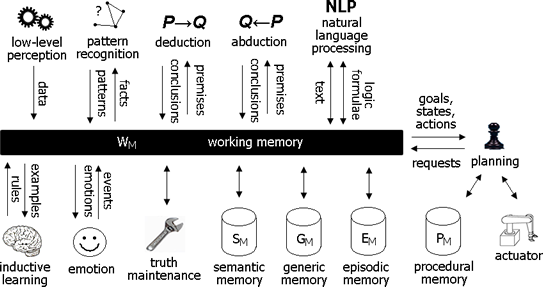
\includegraphics[width=5.65625in,height=2.9895833in,bb=0 0 543 287]{blackboard-architecture.png}
%\caption{AGI architecture}
\end{figure}

Here is a simple top-level algorithm to process incoming sensory events:

\begin{algorithm}[H]
\caption{Top-level sensory processing}
\alginout{raw sensory input}
{updated KB}
\begin{algtab}
\alglabel{alg:top-level-sensory-processing}

Upon the arrival of raw sensory input, perform \textbf{pattern recognition} (\S\ref{ch:pattern-recognition}) which is the same as forward-chaining (\S\ref{sec:deduction}).  (NL input can bypass this step.)  The result will be a set of \textit{new facts} and will be put in Working Memory.  Forward chaining can be performed several times on top of previous results.\\

Perform \textbf{consistency check} (\S\ref{sec:consistency-check}) on the new facts against the KB\\

If a new fact is inconsistent with the current KB, invoke \textbf{conflict resolution} (\S\ref{sec:conflict-resolution})\\

Perform \textbf{abduction} (\S\ref{sec:abduction}) on the new facts, so WM will make appropriate assumptions to account for them.\\

Invoke the \textbf{inductive learner} (\S\ref{sec:inductive-learner}), ie, try to compress the new facts + KB.\\
\end{algtab}
\end{algorithm}
\vspace{-0.6cm}

The abduction algorithm is almost identical to the consistency-check algorithm, so they may be merged.  The abduction algorithm is also very similar to the induction algorithm (cf \S\ref{sec:abduction}), so all 3 may be merged.

\section{BDI architecture}
\index{architecture!BDI architecture}

BDI (\textbf{belief-desire-intention}) is one of the most successful agent architectures ever proposed.  It was first investigated by Michael Bratman as a theory of human practical reasoning (\citep*{Bratman1987}), and later formulated as an agent architecture (\citep*{Bratman1988}).  The main concern of BDI is how to plan in the face of a \textit{dynamic environment} and with \textit{bounded resources}.

Key to BDI is the idea of \textbf{commitment}.  Once an agent commits to a plan, the plan will constrain means-end reasoning, thus making planning processes more efficient.

\textbf{B: Beliefs} are the contents of the KB.\\
\textbf{D: Desires} are unconstrained;  they need not be achievable or even consistent (eg, one can desire smoking and good health at the same time).\\
\textbf{I: Intentions} are goals that the agent commits to;  they are believed to be achievable and must be consistent.

\begin{figure}[t]
\centering
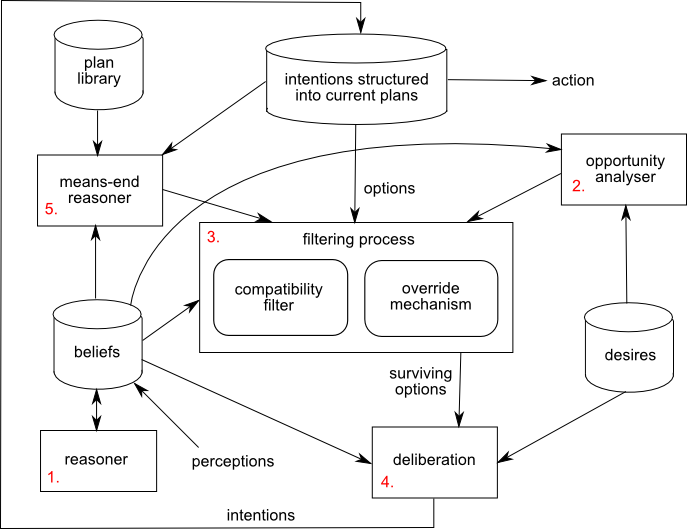
\includegraphics[scale=0.7]{BDI-architecture.png}
\caption{schematic diagram of the BDI architecture}
\label{fig:BDI-arch}
\end{figure}

Figure \ref{fig:BDI-arch} is a schematic diagram of BDI.  The key processing steps are:
\begin{compactenum}
\item  This is the \textbf{Knowledge / Declarative Sub-system}, which we will consider at length in the rest of the book.
\item  Changes in the environment cause changes in beliefs, which in turn reveal new possibilities to satisfy desires.  Thus the \textbf{Opportunity Analyzer} tries to propose new \textbf{options}.
\item  Once the options are produced (either by the Opportunity Analyzer or the Means-end Reasoner), they are subject to \textbf{filtering}.  The \textbf{Compatibility Filter} checks if options are compatible with existing plans.
\item  Surviving options are weighted against each other by the \textbf{Deliberation Process}, which produces intentions to be incorporated as plans.
\item  The \textbf{Means-end Reasoner} searches for the next available options, taking into consideration the current plans.
\end{compactenum}

\section{Evolutionary architecture}

\{ TO-DO:  Hayek is not the correct designation for this architecture \}

Hayek is an artificial economy proposed by Eric Baum (\citep*{Baum2004}) as an AGI architecture.  A slight variant of Hayek can be described as follows:
\index{architecture!Hayek architecture (economic model)}

\begin{compactenum}
\item The AGI is composed of a large number of small programs.
\item \textbf{Cooperativity}.  The programs may call each other.
\item \textbf{Persistent memories}.  Individual programs can remember things across time slices.
\item A \textbf{meta-controller} runs these programs according to some schedule, allotting each program a time slice.
\item \textbf{Credit assignment}:  If the program answers a question correctly or performs a good action (judged by some external critic), the meta-controller will credit the programs that have contributed to the result.
\item Human programmers may contribute to this pool of programs.\\
\end{compactenum}

A high-level programming language (such as Lisp) seems to be more suitable for this purpose.

Note that even very complex algorithms can be implemented in this architecture.  For example, a best-first search algorithm can remember its search state in an external memory store.  Then it just waits for its time-slice to resume searching.  Thus human programmers can seed the artificial economy with highly competent programs.

\section{Decision-theoretic architecture}
\index{architecture!decision-theoretic}

This is mathematically more elegant than the BDI architecture.

Some important elements that should be present in the architecture:
\begin{compactenum}[1.]
\item  \textbf{percepts} are raw (unprocessed) sensory events
\item  \textbf{beliefs} are the contents of the KB
\item  \textbf{states} --- all possible \textit{perceived} states of the environment, including the current state.  States are special terms in the logic.
\item  \textbf{actions}
\item  \textbf{utility function} --- a function $U: \{state\} \rightarrow \mathbb{R}$.  Utilities may be defined implicitly, though.
\\
\end{compactenum}

This architecture may depend on a \textbf{logical sub-system} that:
\begin{compactenum}[1.]
\item  recognizes environmental states (eg \textit{``the apple is on the table''}) from raw percepts (eg pixel values from a camera)
\item  recognizes possible actions (eg \textit{``I can put the apple on the plate''})
\\
\end{compactenum}

The goal is to maximize expected utility.  Planning becomes a discrete optimization problem in this setting.

Reinforcement learning \index{reinforcement learning} can be naturally included in this architecture.

\section{Self-programming architecture}
\label{sec:self-programming-architecture}
\index{architecture!self-programming}
\index{programming!self-programming}

Consider this variant of the chicken-and-egg problem (\S\ref{sec:chicken-and-egg}), where we distinguish between the \textbf{Synthesizer} and the AGI:
\begin{figure}[H]
\centering
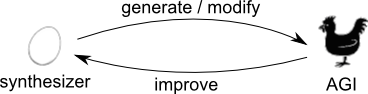
\includegraphics{self-programming-architecture.png}
%\caption{improved self-programming architecture}
\vspace{-0.5cm}
\end{figure}

Currently we know the following program-synthesis paradigms:\\
1.  human programming\\
2.  natural reasoning (NR), ie common-sense / human-like reasoning\\
3.  automated theorem proving (ATP)\\
4.  stochastic local search (SLS), including evolutionary algorithms (EA)\\
5.  reinforcement learning (RL) \index{reinforcement learning}\\
We will consider each paradigm in turn.

A key question is how an initially-dumb AGI can \textit{improve} the performance of the Synthesizer, even slightly.

\textbf{1. Human programming} (ie, brute-force software engineering without RSI)\\ \index{programming!human}
The problem with this approach is that it does not exploit the advantages of machine program synthesis, and thus is likely to be sub-optimal.

\textbf{2. Natural reasoning} (cf \S\ref{sec:natural-reasoning})
\begin{compactenum}[(a)]
\item  The problem is that NR does not yet exist, but it is a \textit{sine-qua-non desideratum} of AGI.
\item  So the question is how to enable an initially weak form of NR to synthesize programs.  One possibility is to use \textbf{creativity}:  the AGI will generate programs by partly reasoning and partly random acting.
\item  An agent with NR is likely to have RL as well.
\item  An NR agent can invoke ATP.
\item  An NR agent can self-program (without invoking ATP), simply by \textbf{deductive planning} (\S\ref{sec:deductive-planning}).\\
\end{compactenum}

\textbf{3. ATP} \index{programming!ATP (automated theorem proving)}
\begin{compactenum}[(a)]
\item  It requires \textit{formal} specifications of programs (or sub-routines), which are often very hard to write for humans.
\item  Search in proof space can be very slow.
\item  There already exists ATP-based program synthesis software, which can be used externally.\\
\end{compactenum}

\textbf{4. Stochastic local search} \index{search!stochastic local search}
\begin{compactenum}[(a)]
\item  Is based on generate-and-test.
\item  ``Generate'' is random and the program space is typically huge.
\item  ``Test'' is often slow because it requires the entire AGI to answer a large number of benchmark queries.  A possible remedy is to specify input-out benchmarks for AGI \textit{components}, but then the burden is on humans to design the modular architecture.
\item  A large population of relatively low-score programs has to be maintained, in order to allow sufficient time for cooperativity to evolve.  For this reason I suspect that the evolutionary approach is rather slow.
\item  2 further problems are:  How can an initially-dumb AGI improve the stochastic searcher?\footnote{In MOSES (cite) an attempt is made at ``representation building''.} And how can this transfer of rationality from the AGI to the Synthesizer be coded once and for all?\\
\end{compactenum}

\textbf{5. Reinforcement learning} \index{reinforcement learning}
\begin{compactenum}[(a)]
\item  The goal of RL is to learn policies of how to act in certain environmental states.  It can synthesize programs if the environment is that of programming.
\item  RL can be augmented with logical reasoning.
\item  RL can implement the idea of expected utility maximization.
\\
\end{compactenum}

\textbf{Combining all methods}\\
Apparently, we can combine all the above methodologies without conflict:
\begin{figure}[H]
\centering
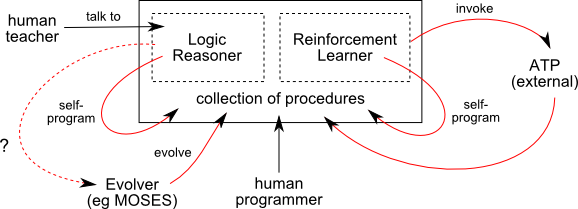
\includegraphics{combined-architecture.png}
\vspace{-0.5cm}
\end{figure}

The question is to choose the \textit{most effective} method of AGI self-programming (red lines).  My intuition is that the evolutionary method is much less efficient than the other 3 (it is easier to explain to children to do something than to train animals by reinforcement, which is in turn easier than breeding animals for the innate ability to do that thing), provided that some rudimentary ability of reasoning is present.

Maybe the most cost-effective method (from the human labor perspective) is to combine RL with logical reasoning and deductive planning --- for instance, to allow RL to invoke IE (inference engine) or vice versa.

\section{AIXI}

\section{Distributive architecture}
